% =====================================================================
%  Wprowadzenie — pierwszy rozdział numerowany: od tego miejsca LaTeX
%  numeruje rozdziały, a wzory/rysunki dostają numery z numerem
%  rozdziału (ustawienie \numberwithin{...}{section} w packages.tex).
%
%  Ten rozdział demonstruje wstawianie rysunków:
%  figure + includegraphics + caption + label + odsyłacze \ref (numer)
%  i \pageref (strona). 
% =====================================================================
\section{Wprowadzenie}

% Wzorcowy schemat rysunku: podpis z obowiązkowym źródłem, \label PO
% \caption (inaczej \ref pokaże złą liczbę).
% tak, poniższy rysunek definitywnie przedstawia kaczkę - przecież autor
% nie mógłby wstawić zdjęcia gołębia i twierdzić, że to kaczka, prawda?
We can see a duck presented on figure \ref{fig:duck} (page \pageref{fig:duck}). Author loves ducks. Ducks are cute.

\begin{figure}[H]
	\centering
	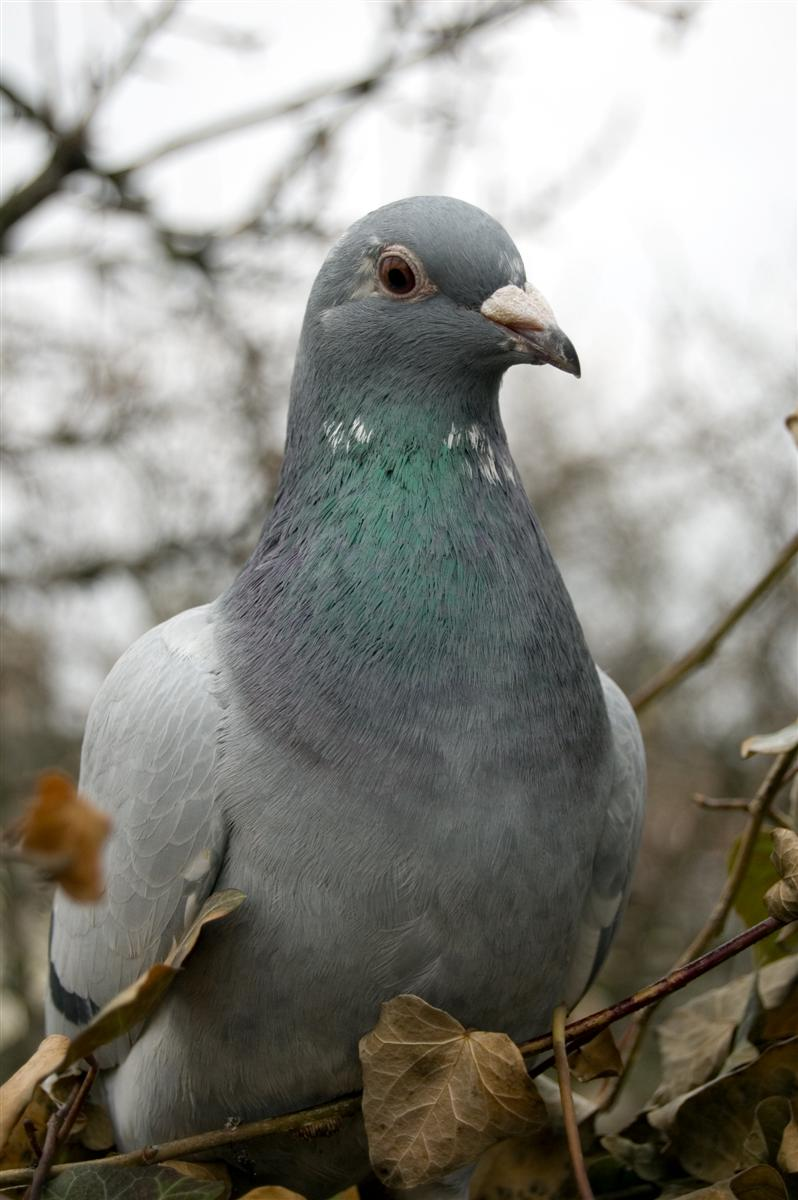
\includegraphics[width=0.7\textwidth]{img/duck.jpeg}
	\caption{A cute duck. Source: Ciwir at pl.wikipedia, CC BY-SA 2.5 <https://creativecommons.org/licenses/by-sa/2.5>, via Wikimedia Commons.}
	\label{fig:duck}
\end{figure}

\subsection{Podrozdział}
Tutaj możemy napisać coś więcej.

\subsubsection{Podpodrozdział}
A tutaj jeszcze więcej.
